\chapter{Evaluation on publicly available datasets}\label{chap:toy-dataset}

The three loss functions presented in chapter \ref{chap:clustering-metric} were  experimentally evaluated on publicly available datasets.

\section{Used datasets}

The evaluation was done on a set of 20 datasets. These are, in alphabetical order:
\begin{enumerate}
  \item The "BrownCreeper" and "WinterWren" datasets. See \cite{briggs_rank-loss_2012}. A dataset of bird songs where each bag represents a recording of one or multiple birds. Originally a 13-class dataset, converted to binary classification datasets by selecting a target class.
  \item The "CorelAfrican" and "CorelBeach" datasets. See \cite{chen_miles:_2006}. A dataset of object images where each bag is an image, consisting of segments described by \( 4 \times 4 \) patch features. Originally a 20-class dataset, converted to binary classification datasets by selecting a target class.
  \item The "Elephant", "Fox" and "Tiger" datasets. See \cite{andrews_support_2002}. A dataset of animal images where each bag is an image, consisting of segments. Originally a multi-class dataset (also with animals other that the 3), converted to binary classification datasets by selecting a target class.
  \item The "Musk1" and "Musk2" datasets. See \cite{dietterich_solving_1997}. A dataset of molecules where each bag is a set of the different shapes the molecule can fold into (so-called \textit{conformers}). The goal is to predict whether a molecule has a musky smell or not. If at least one of the conformers of a molecule can cause it to smell musky, the molecule is positive.
  \item The "Mutagenesis1" and "Mutagenesis2" datasets. See \cite{srinivasan_comparing_1995}. A dataset consisting of a drug activity prediction problem. There is an easy ("Mutagenesis1") and a hard ("Mutagenesis2") version.
  \item The "Newsgroups1", "Newsgroups2" and "Newsgroups3" datasets. See \cite{zhou_multi-instance_2008}. A text categorization dataset where each bag is a collection of posts from different newsgroups. A positive bag for a class is designed to contain 3\% of posts from the target class and 97\% randomly sampled from the other categories. Originally a 20-class dataset, converted to binary classification datasets by selecting a target class.
  \item The "Protein" dataset. See \cite{ray_learning_2005} and \cite{ray_supervised_2005}. A dataset consisting of protein annotations making it a text categorization problem. The task is to decide whether a given pair should be annotated by a Gene Ontology (GO) code.
  \item The "UCSBBreastCancer" dataset. See \cite{kandemir_empowering_2014}. A dataset consisting of 38 TMA image excerpts from breast cancer patients where each bag represents an image excerpt consisting of image patches. The goal is to predict whether the cancer is benign or malignant.
  \item The "Web1", "Web2", "Web3" and "Web4" datasets. See \cite{zhou_multi-instance_2005}. A dataset of webpages as ranked by 4 different users based on their being interesting. Each bag represents a webpage with instances being the links on the webpage.
\end{enumerate}

All the datasets as used were made public in \cite{dedic_mildatasetsjl_2019}.

\section{Used models}

The models for evaluation were implemented in the Julia programming language (see \cite{bezanson_julia:_2017}) using the Flux.jl framework for machine learning (see \cite{innes_flux:_2018}) and the Mill.jl framework for multi-instance learning (see \cite{pevny_milljl_2019}).

The embedding \( \phi \) was realised by a MIL neural network consisting of 2 per-instance layers of 30 neurons, followed by aggregation formed by concatenating element-wise mean and element-wise maximum of all instances in a bag, followed by 2 per-bag layers of 30 neurons. All the neurons used the ReLU activation function (see \cite{hahnloser_digital_2000}). Layer weights were initialized using Glorot initialization (see \cite{glorot_understanding_2010}), bias vectors were initialized to zeros. ADAM (see \cite{kingma_adam:_2014}) was used as the optimization method.

For each of the datasets, 80\% of bags was randomly chosen as the training data, with the rest being testing data. The models were trained using 100 mini-batches of size 50.

\section{Mean model and classification model}\label{sec:baseline-models}

In order to provide some baseline against which the models could be compared (as there is no prior art for this problem), two other models were introduced.

A non-machine-learning model was introduced as a baseline, which all models should surpass. This model implements the embedding \( \phi \) as an element-wise mean of all instances of a bag.

A classification model has been introduced as a target to beat. This model was realised by a MIL neural network consisting of 2 per-instance layers of 30 neurons, followed by aggregation formed by concatenating element-wise mean and element-wise maximum of all instances in a bag, followed by 2 per-bag layers of 30 neurons and a final layer of 2 output neurons. All the neurons used the ReLU activation function, except for the output neurons which used identity as their activation function. Layer weights were initialized using Glorot initialization, bias vectors were initialized to zeros. ADAM was used as the optimization method optimizing the cross-entropy loss. The accuracy of the model has been evaluated by selecting the optimal threshold on its output.

\section{Method hyper-parameter selection}

Some of the three proposed clustering-losses have some hyper-parameters which need to be tuned. \( L_\mathrm{CPC} \) has no hyper-parameters, \( L_\mathrm{triplet} \) has a single hyper-parameter \( c \), and \( L_\mathrm{magnet} \) has three hyper-parameters, \( K \), \( \alpha \) and the cluster index update frequency. For \( L_\mathrm{triplet} \) and \( L_\mathrm{magnet} \), a range of values was tried for each hyper-parameter in order to select the best configuration for each. The testing was done on the "Musk2" dataset, as it is sufficiently hard and simultaneously the best-known industry standard dataset for MIL.

\subsection{Triplet loss}
For \( L_\mathrm{triplet} \), the values \( c \in \left\{ 0.01, 0.1, 1, 10, 100 \right\} \) have been tested. Figure \ref{fig:triplet-gridsearch-ratio} shows the values of \( \mathrm{ratio} \left( \cdot \right) \) (see section \ref{sec:clustering-metrics}) for the different hyper-parameter values, figure \ref{fig:triplet-gridsearch-accuracy} shows the accuracy of a kNN classifier built on the embedding.

\begin{figure}[h]
  \centering
  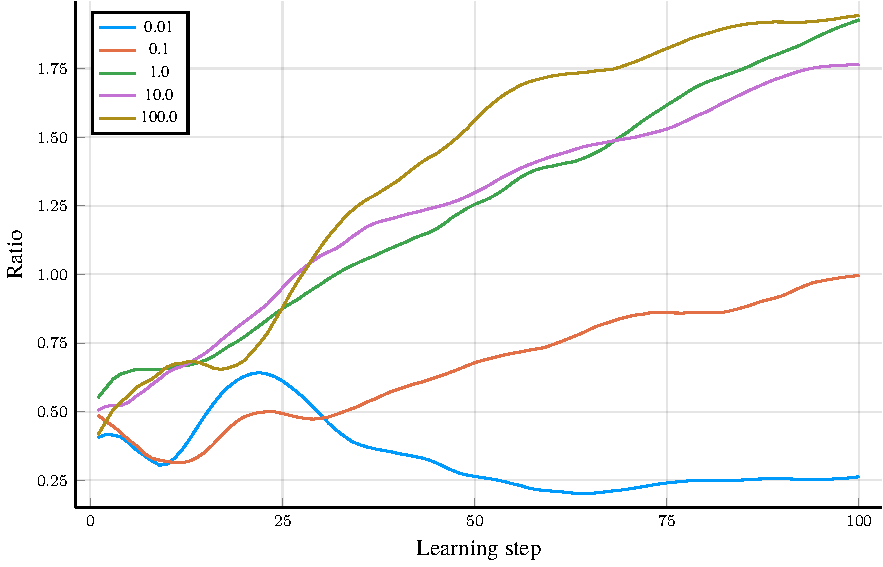
\includegraphics[width=\textwidth]{images/triplet-gridsearch/ratio/triplet-gridsearch-ratio.pdf}
  \caption{The value of \( \mathrm{ratio} \left( \cdot \right) \) over the learning period for triplet loss.}\label{fig:triplet-gridsearch-ratio}
\end{figure}

\begin{figure}[h]
  \centering
  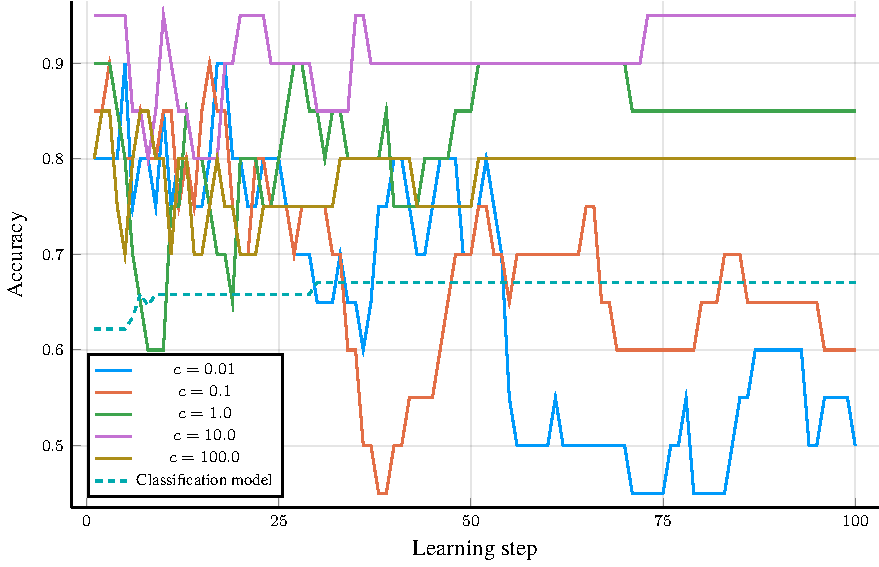
\includegraphics[width=\textwidth]{images/triplet-gridsearch/accuracy/triplet-gridsearch-accuracy.pdf}
  \caption{The accuracy of a kNN classifier built on the embedding over the learning period for triplet loss.}\label{fig:triplet-gridsearch-accuracy}
\end{figure}

As can be seen from the figures, for low values of \( c \), the performance is not good and, more importantly, isn't increasing over the learning period. In the end, the value \( c = 1 \) has been selected as it offers good performance and the higher values show some instability in the learning process.

\subsection{Magnet loss}
For \( L_\mathrm{magnet} \), the values \( K \in \left\{ 2, 3, 5, 8, 16, 20 \right\} \), \( \alpha \in \left\{ 0, 0.1, 0.5, 1, 10 \right\} \) and the cluster index update frequency in \( \left\{ 5, 10, 25, 70, 130, 200, 1000 \right\} \) have been tested. Figure \ref{fig:magnet-gridsearch-ratio} shows the values of \( \mathrm{ratio} \left( \cdot \right) \) for the different hyper-parameter values, figure \ref{fig:magnet-gridsearch-accuracy} shows the accuracy of a kNN classifier built on the embedding.

\begin{figure}[h]
  \centering
  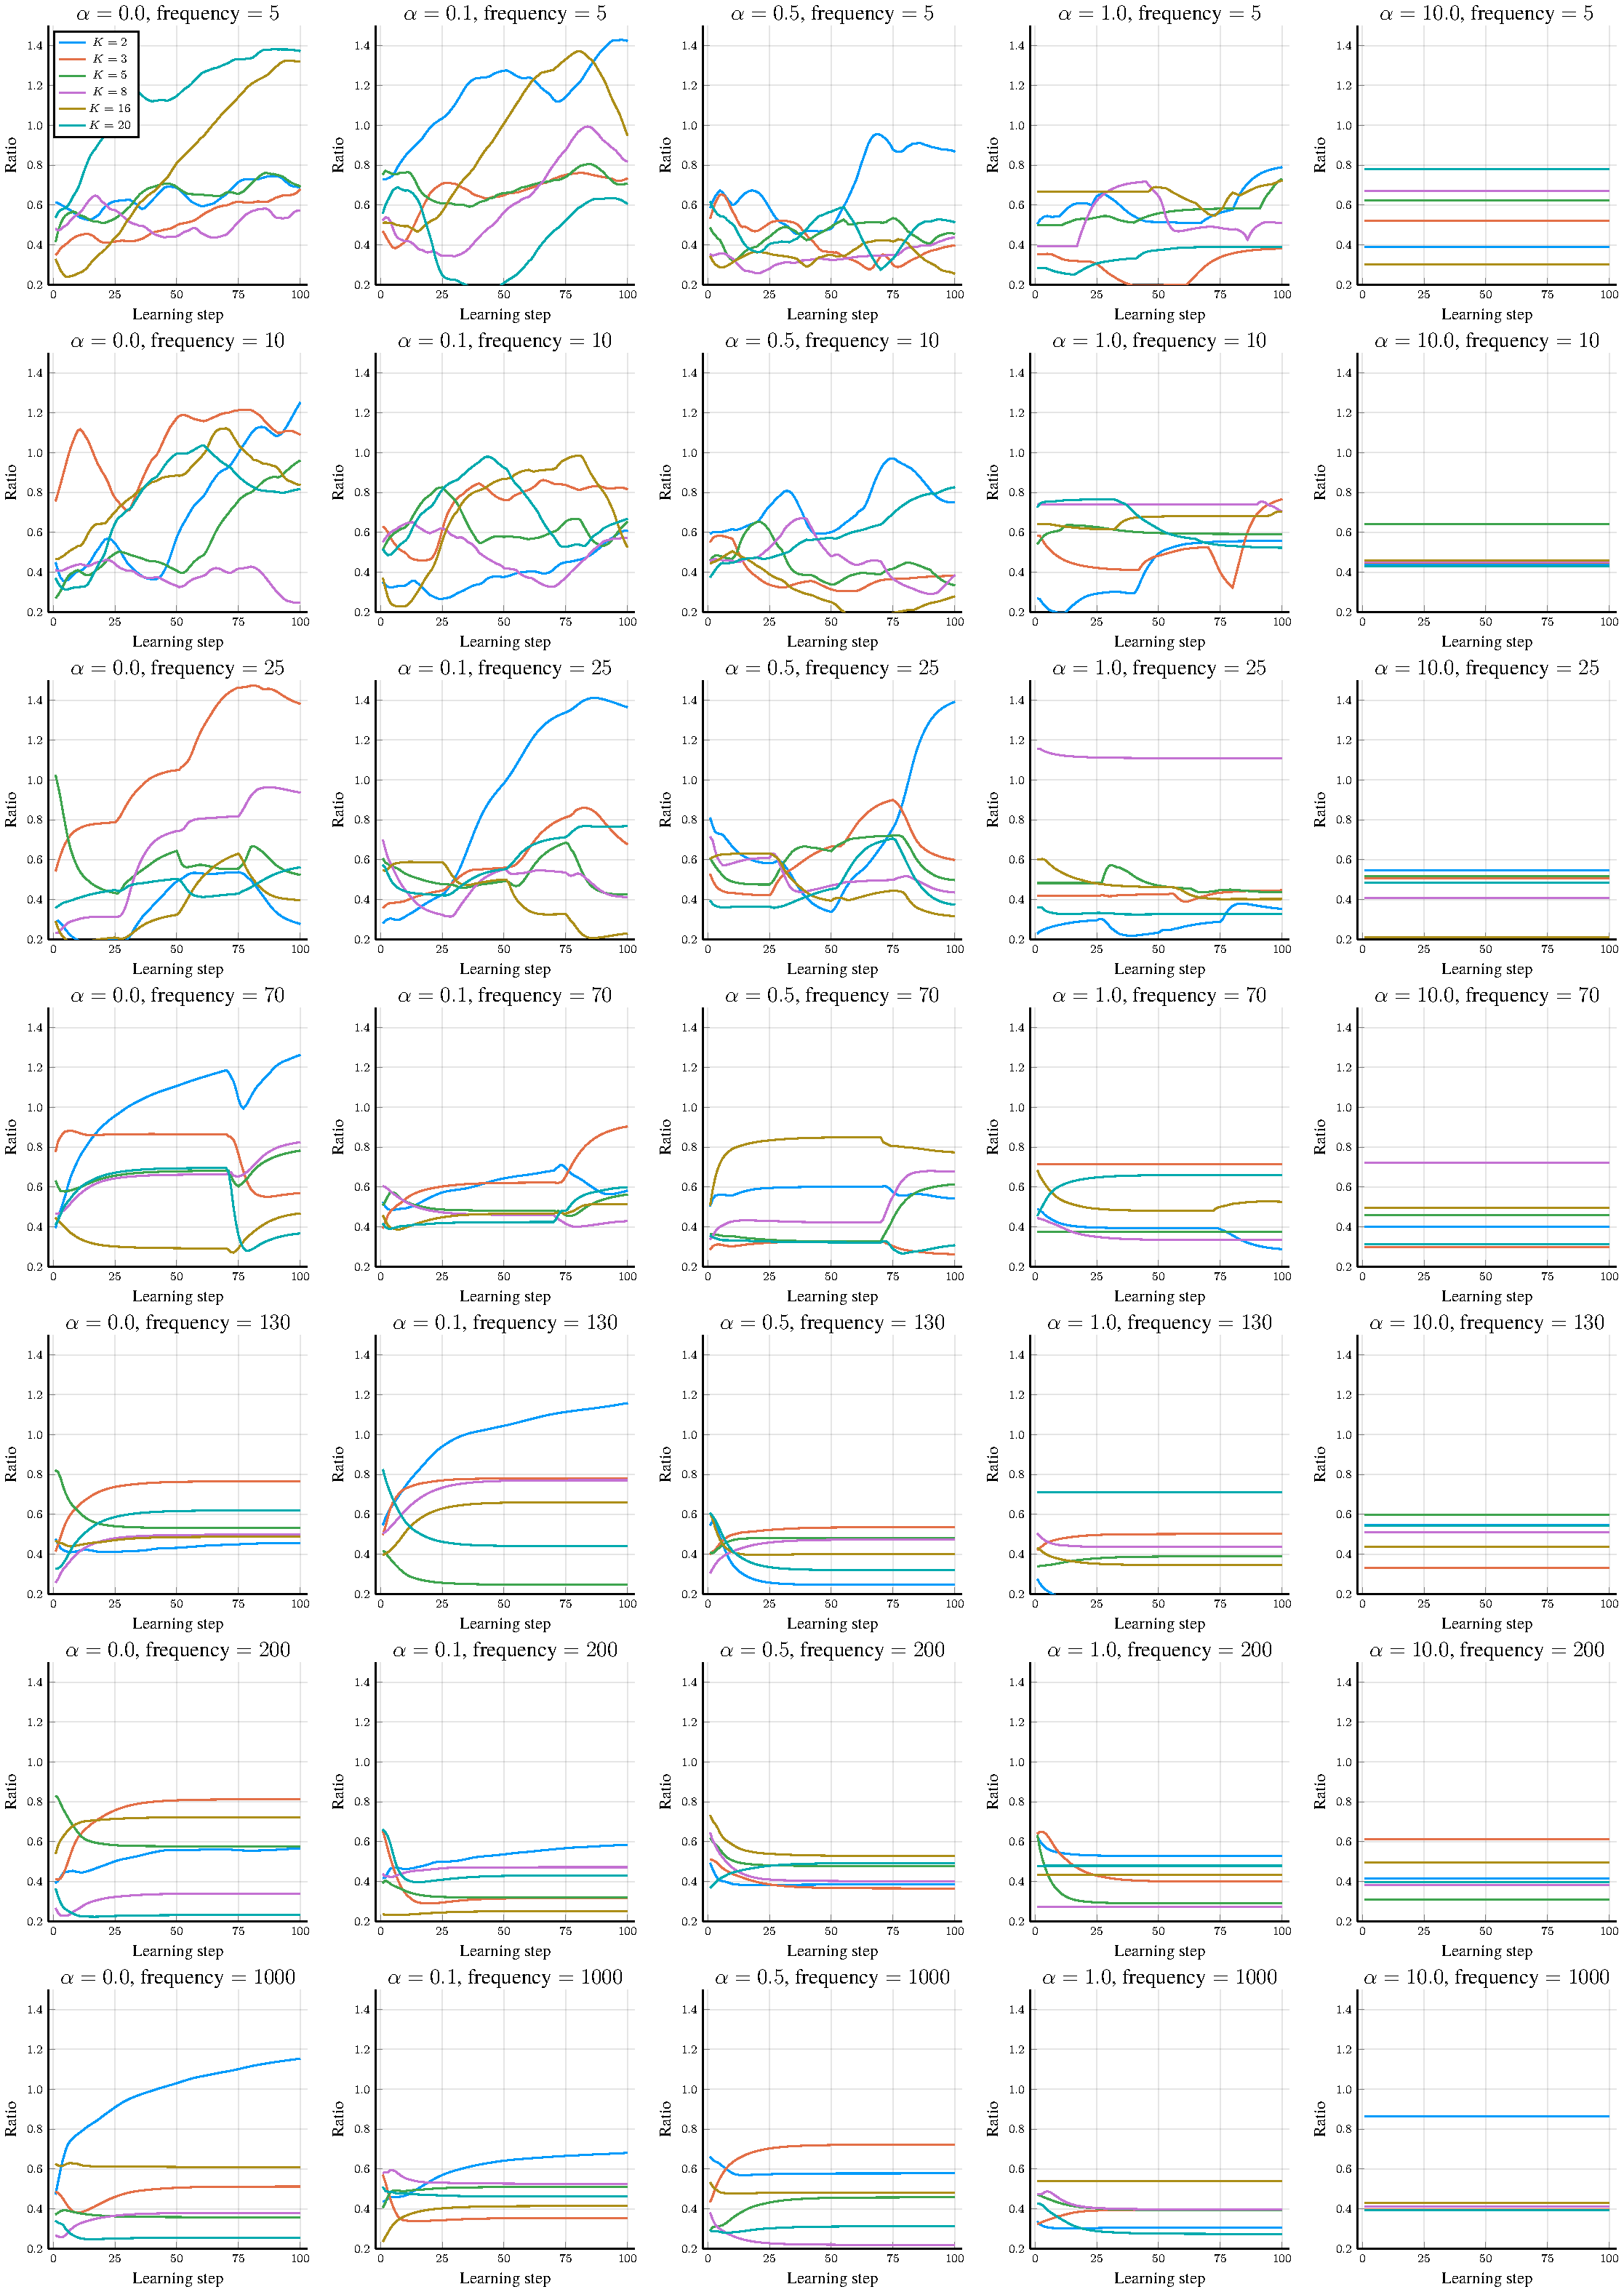
\includegraphics[width=0.93\textwidth]{images/magnet-gridsearch/ratio/K/magnet-gridsearch-ratio-K.pdf}
  \caption{The value of \( \mathrm{ratio} \left( \cdot \right) \) over the learning period for different values of \( K \), \( \alpha \) and the cluster index update frequency. Each subplot corresponds to a particular \( \alpha \) and the cluster index update frequency. The series in each subplot correspond to a value of \( K \).}\label{fig:magnet-gridsearch-ratio}
\end{figure}

\begin{figure}[h]
  \centering
  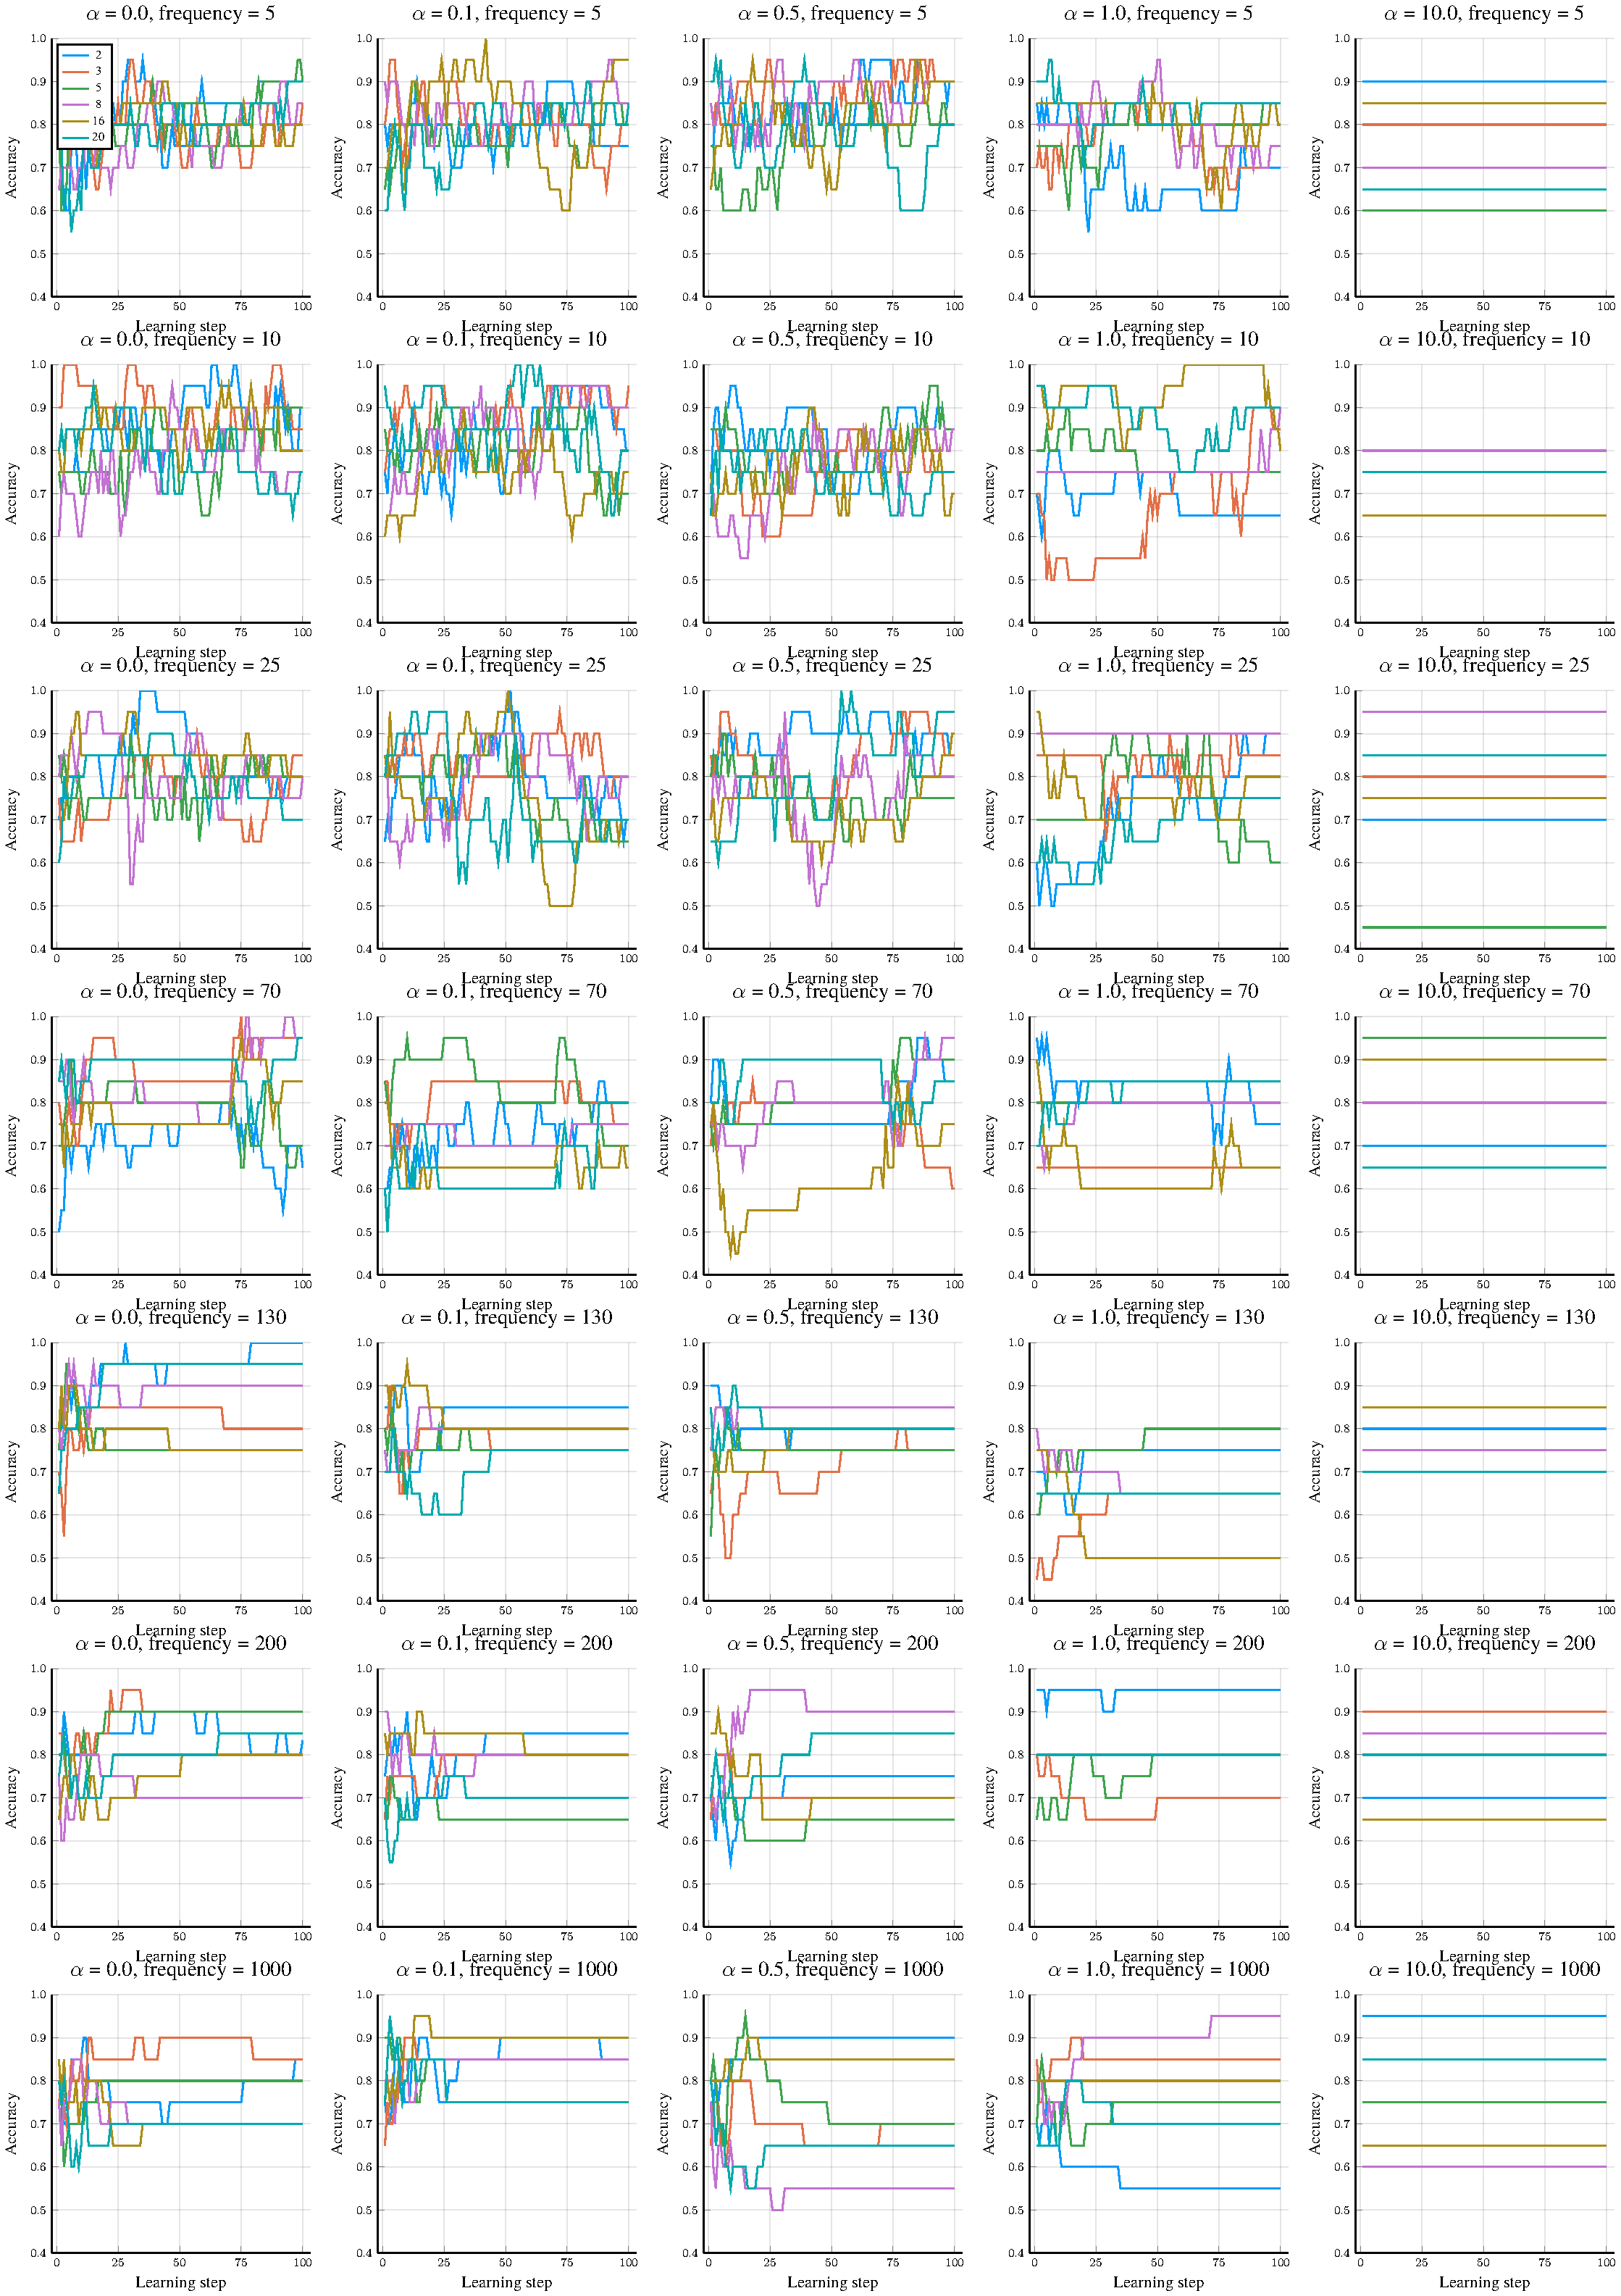
\includegraphics[width=0.93\textwidth]{images/magnet-gridsearch/accuracy/K/magnet-gridsearch-accuracy-K.pdf}
  \caption{The accuracy of a kNN classifier built on the embedding over the learning period for different values of \( K \), \( \alpha \) and the cluster index update frequency. Each subplot corresponds to a particular \( \alpha \) and the cluster index update frequency. The series in each subplot correspond to a value of \( K \).}\label{fig:magnet-gridsearch-accuracy}
\end{figure}

As can be seen from the figures, the value of \( K \) doesn't affect the performance, therefore \( K = 2 \) was chosen due to its lowest computational complexity. For the values of \( \alpha \), the lower values offer better performance, with the values \( 0 \) and \( 0.1 \) being practically indistinguishable. Therefore \( \alpha = 0 \) was chosen. The cluster index update frequency offers no practical change in performance for values up to \( 25 \), with higher values having a negative impact. Therefore, due to computational constraints, the value of \( 25 \) was chosen. The selected hyper-parameter configuration is compared to the mean model and the classification model on the "Musk2" dataset in figure \ref{fig:magnet-baseline}.

\begin{figure}[h]
  \centering
  \begin{subfigure}[b]{0.49\textwidth}
    \centering
    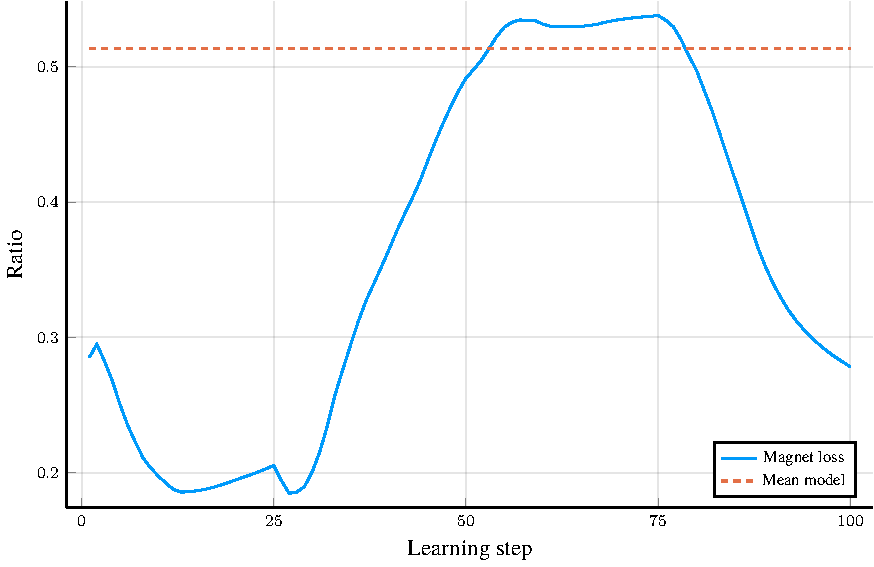
\includegraphics[width=\textwidth]{images/magnet-baseline/ratio/magnet-baseline-ratio.pdf}
    \caption{The value of \( \mathrm{ratio} \left( \cdot \right) \) over the learning period.}
  \end{subfigure}
  \hfill
  \begin{subfigure}[b]{0.49\textwidth}
    \centering
    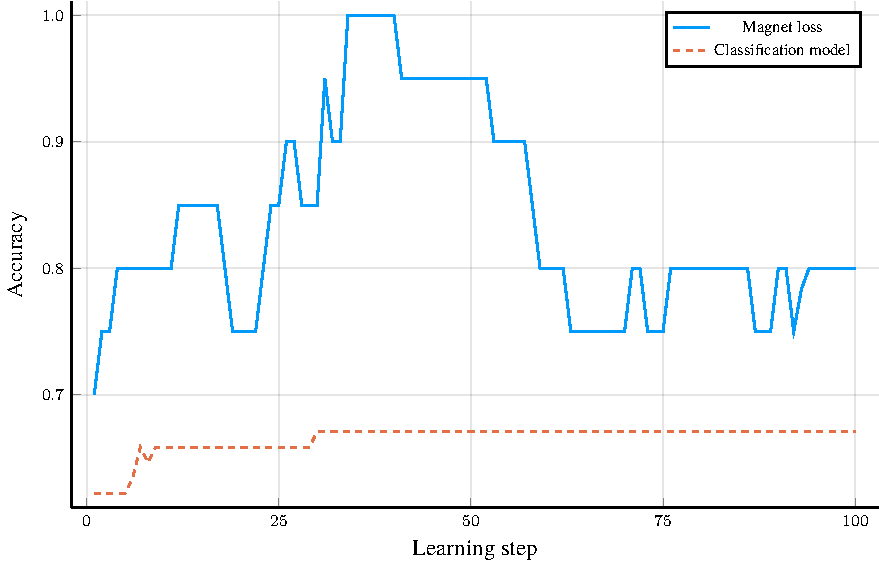
\includegraphics[width=\textwidth]{images/magnet-baseline/accuracy/magnet-baseline-accuracy.pdf}
    \caption{The accuracy of a kNN classifier built on the embedding over the learning period.}
  \end{subfigure}
  \caption{Comparison of the selected hyper-parameter configuration for magnet loss to the mean model and the classification model.}\label{fig:magnet-baseline}
\end{figure}

\section{Method comparison}
The three methods were compared using their best hyper-parameter configuration. All of the methods were evaluated on all of the datasets.

Figure \ref{fig:CPC-toy-ratio} shows the value of \( \mathrm{ratio} \left( \cdot \right) \) for \( L_\mathrm{CPC} \) over the learning period. Figures \ref{fig:CPC-toy-accuracy} and \ref{fig:CPC-toy-kNN} show the accuracy of a kNN model built on the embedding.

\begin{figure}[h]
  \centering
  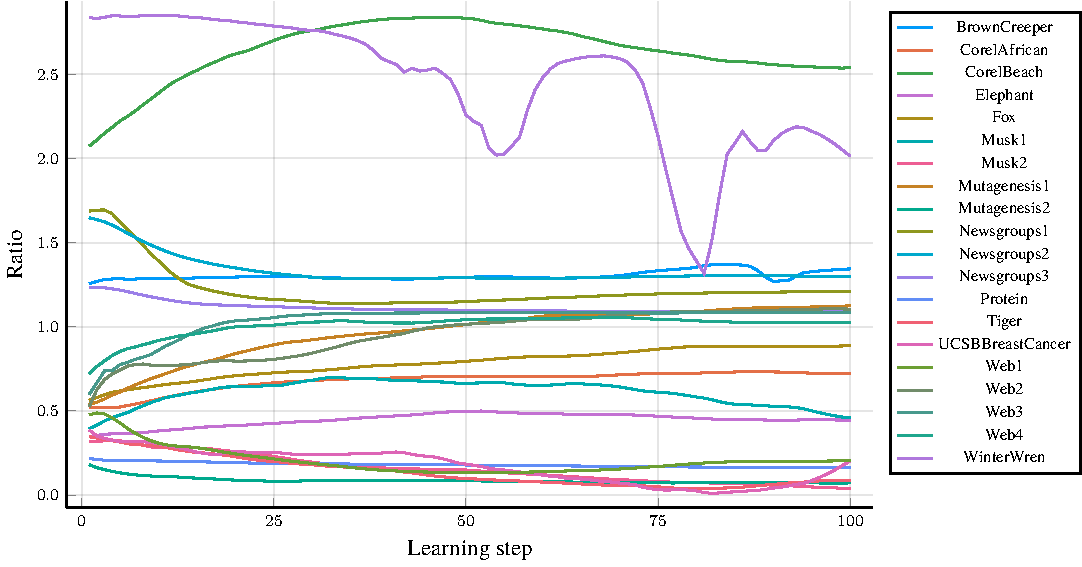
\includegraphics[width=\textwidth]{images/CPC-toy/ratio/CPC-toy-ratio.pdf}
  \caption{The value of \( \mathrm{ratio} \left( \cdot \right) \) for \( L_\mathrm{CPC} \) over the learning period.}\label{fig:CPC-toy-ratio}
\end{figure}

\begin{figure}[h]
  \centering
  \begin{subfigure}[b]{0.49\textwidth}
    \centering
    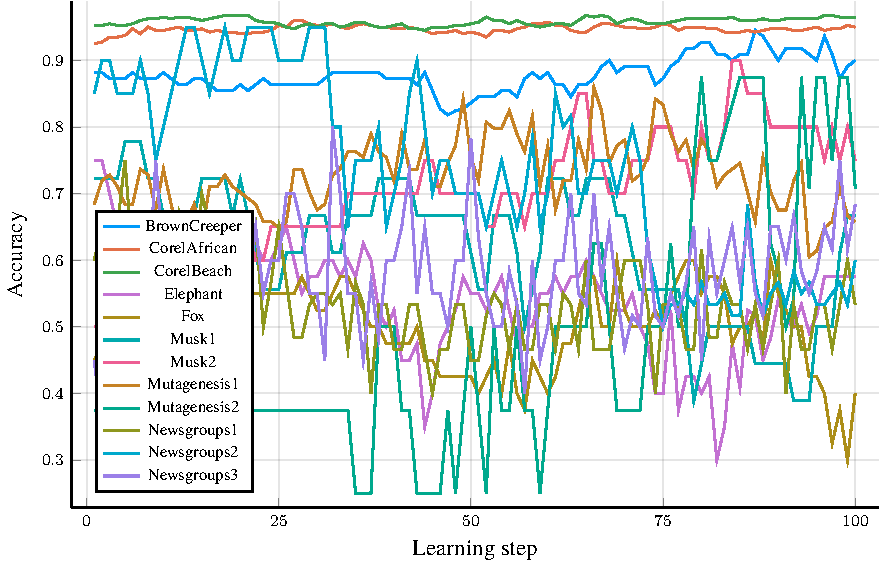
\includegraphics[width=\textwidth]{images/CPC-toy/accuracy1/CPC-toy-accuracy1.pdf}
  \end{subfigure}
  \hfill
  \begin{subfigure}[b]{0.49\textwidth}
    \centering
    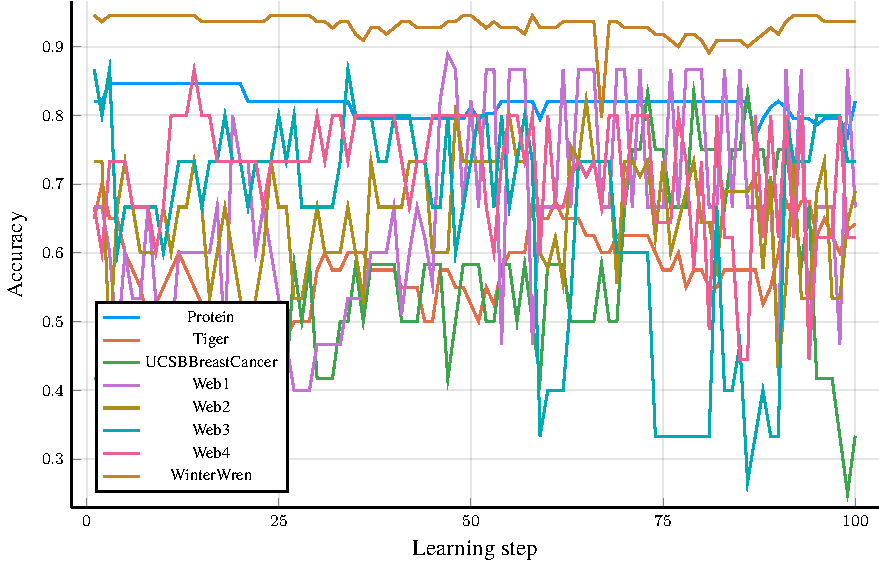
\includegraphics[width=\textwidth]{images/CPC-toy/accuracy2/CPC-toy-accuracy2.pdf}
  \end{subfigure}
  \caption{The accuracy of a kNN classifier built on the embedding for \( L_\mathrm{CPC} \) over the learning period.}\label{fig:CPC-toy-accuracy}
\end{figure}

\begin{figure}[h]
  \centering
  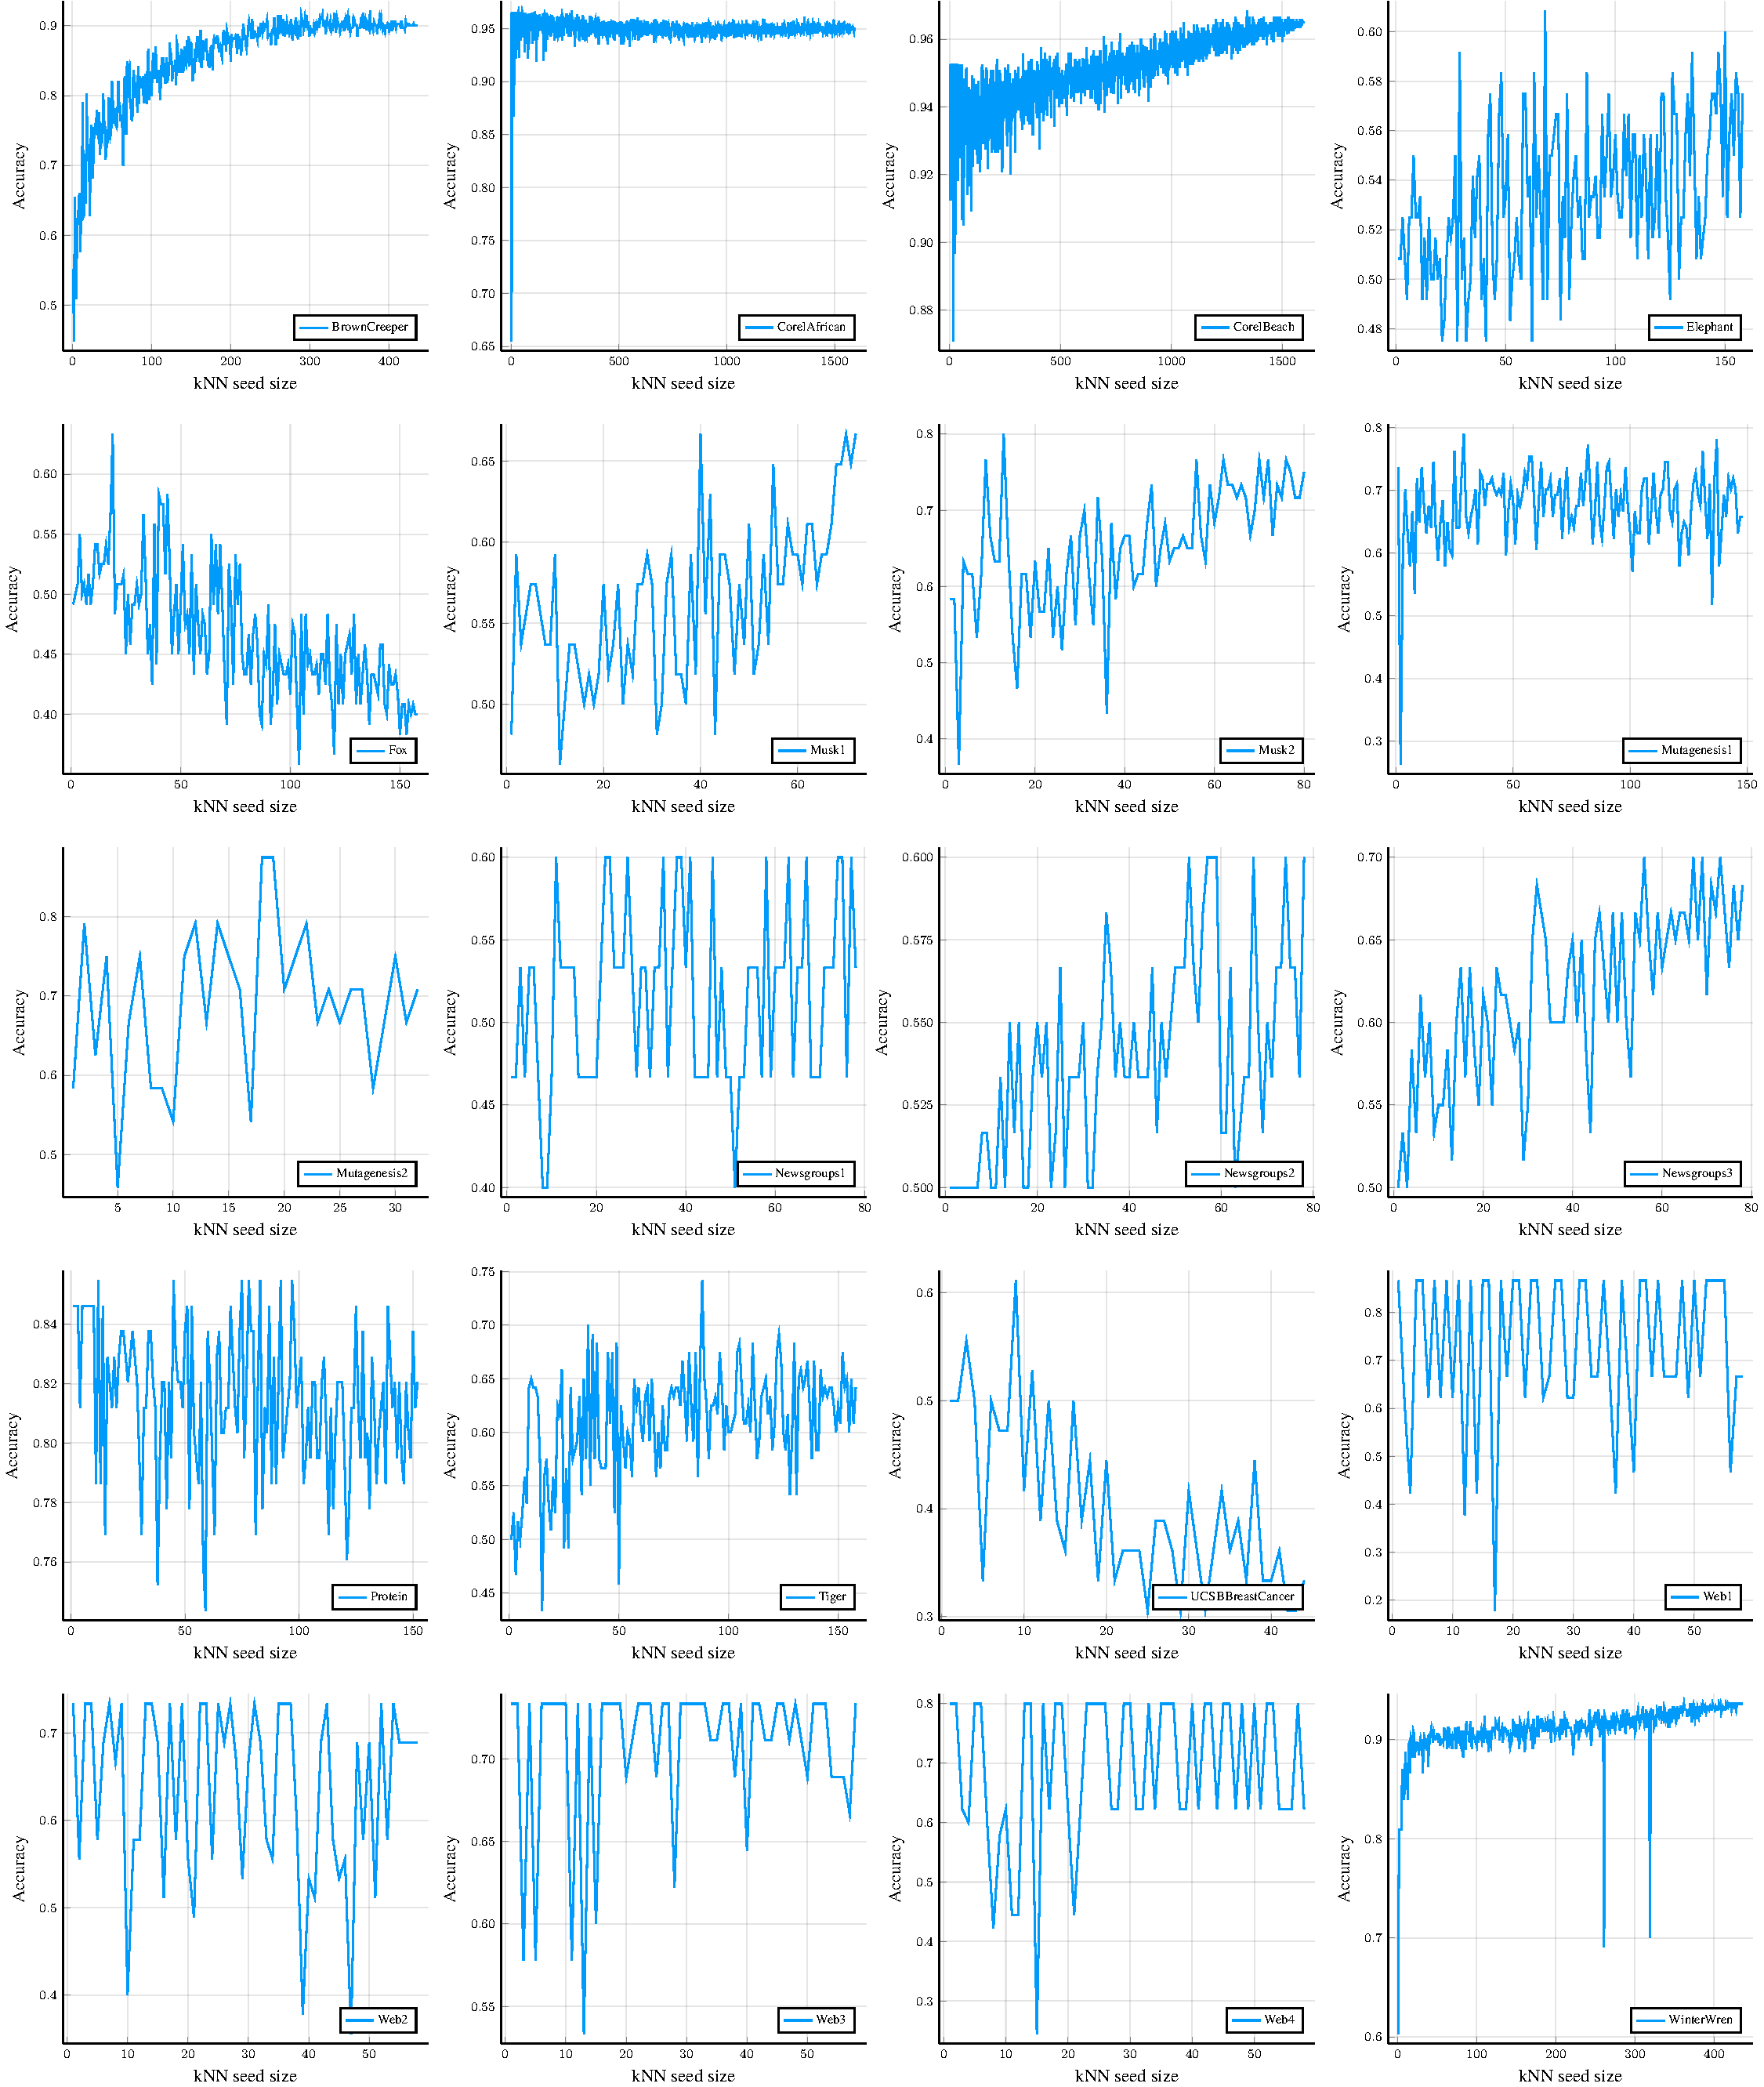
\includegraphics[width=\textwidth]{images/CPC-toy/kNN/CPC-toy-kNN.pdf}
  \caption{The accuracy of a kNN classifier built on the final embedding for \( L_\mathrm{CPC} \) as a function of the number of samples used to seed it. Average of three runs.}\label{fig:CPC-toy-kNN}
\end{figure}

Figure \ref{fig:triplet-toy-ratio} shows the value of \( \mathrm{ratio} \left( \cdot \right) \) for triplet loss over the learning period. Figures \ref{fig:triplet-toy-accuracy} and \ref{fig:triplet-toy-kNN} show the accuracy of a kNN model built on the embedding.

\begin{figure}[h]
  \centering
  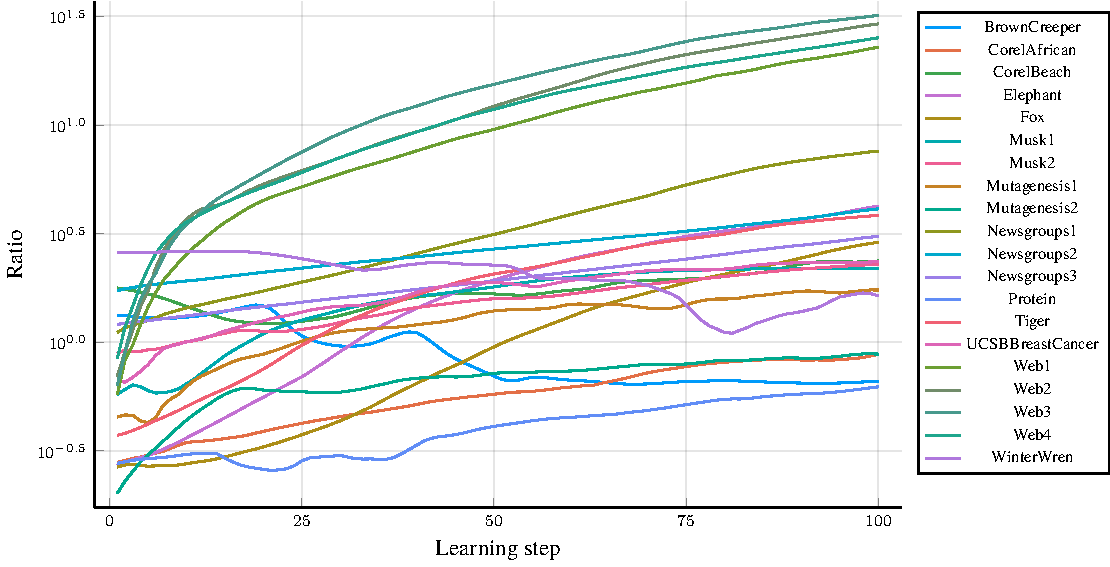
\includegraphics[width=\textwidth]{images/triplet-toy/ratio/triplet-toy-ratio.pdf}
  \caption{The value of \( \mathrm{ratio} \left( \cdot \right) \) for triplet loss over the learning period. Note the logarithmic scale on the \( y \) axis.}\label{fig:triplet-toy-ratio}
\end{figure}

\begin{figure}[h]
  \centering
  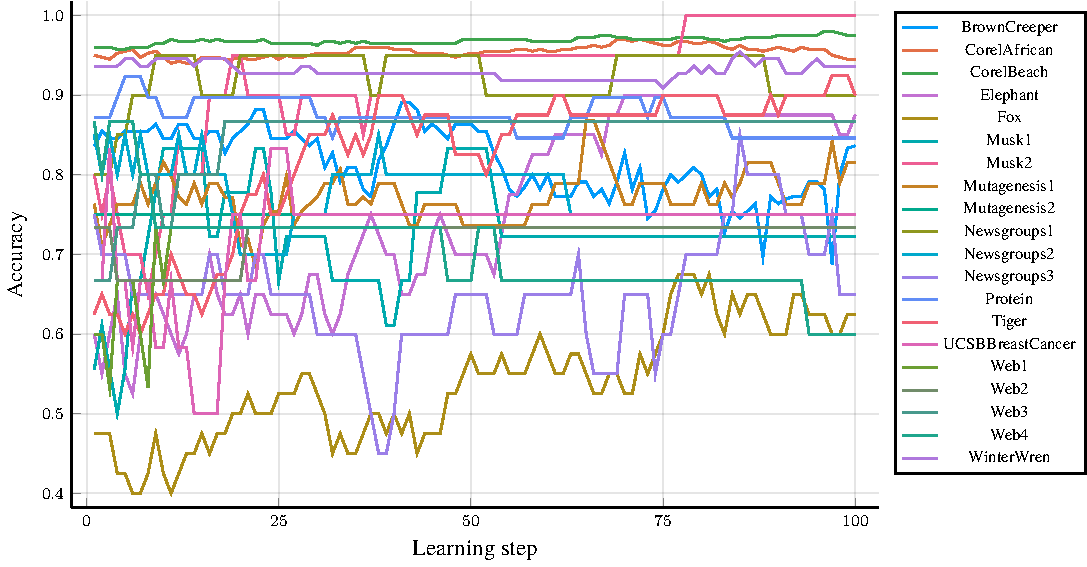
\includegraphics[width=\textwidth]{images/triplet-toy/accuracy/triplet-toy-accuracy.pdf}
  \caption{The accuracy of a kNN classifier built on the embedding for triplet loss over the learning period.}\label{fig:triplet-toy-accuracy}
\end{figure}

\begin{figure}[h]
  \centering
  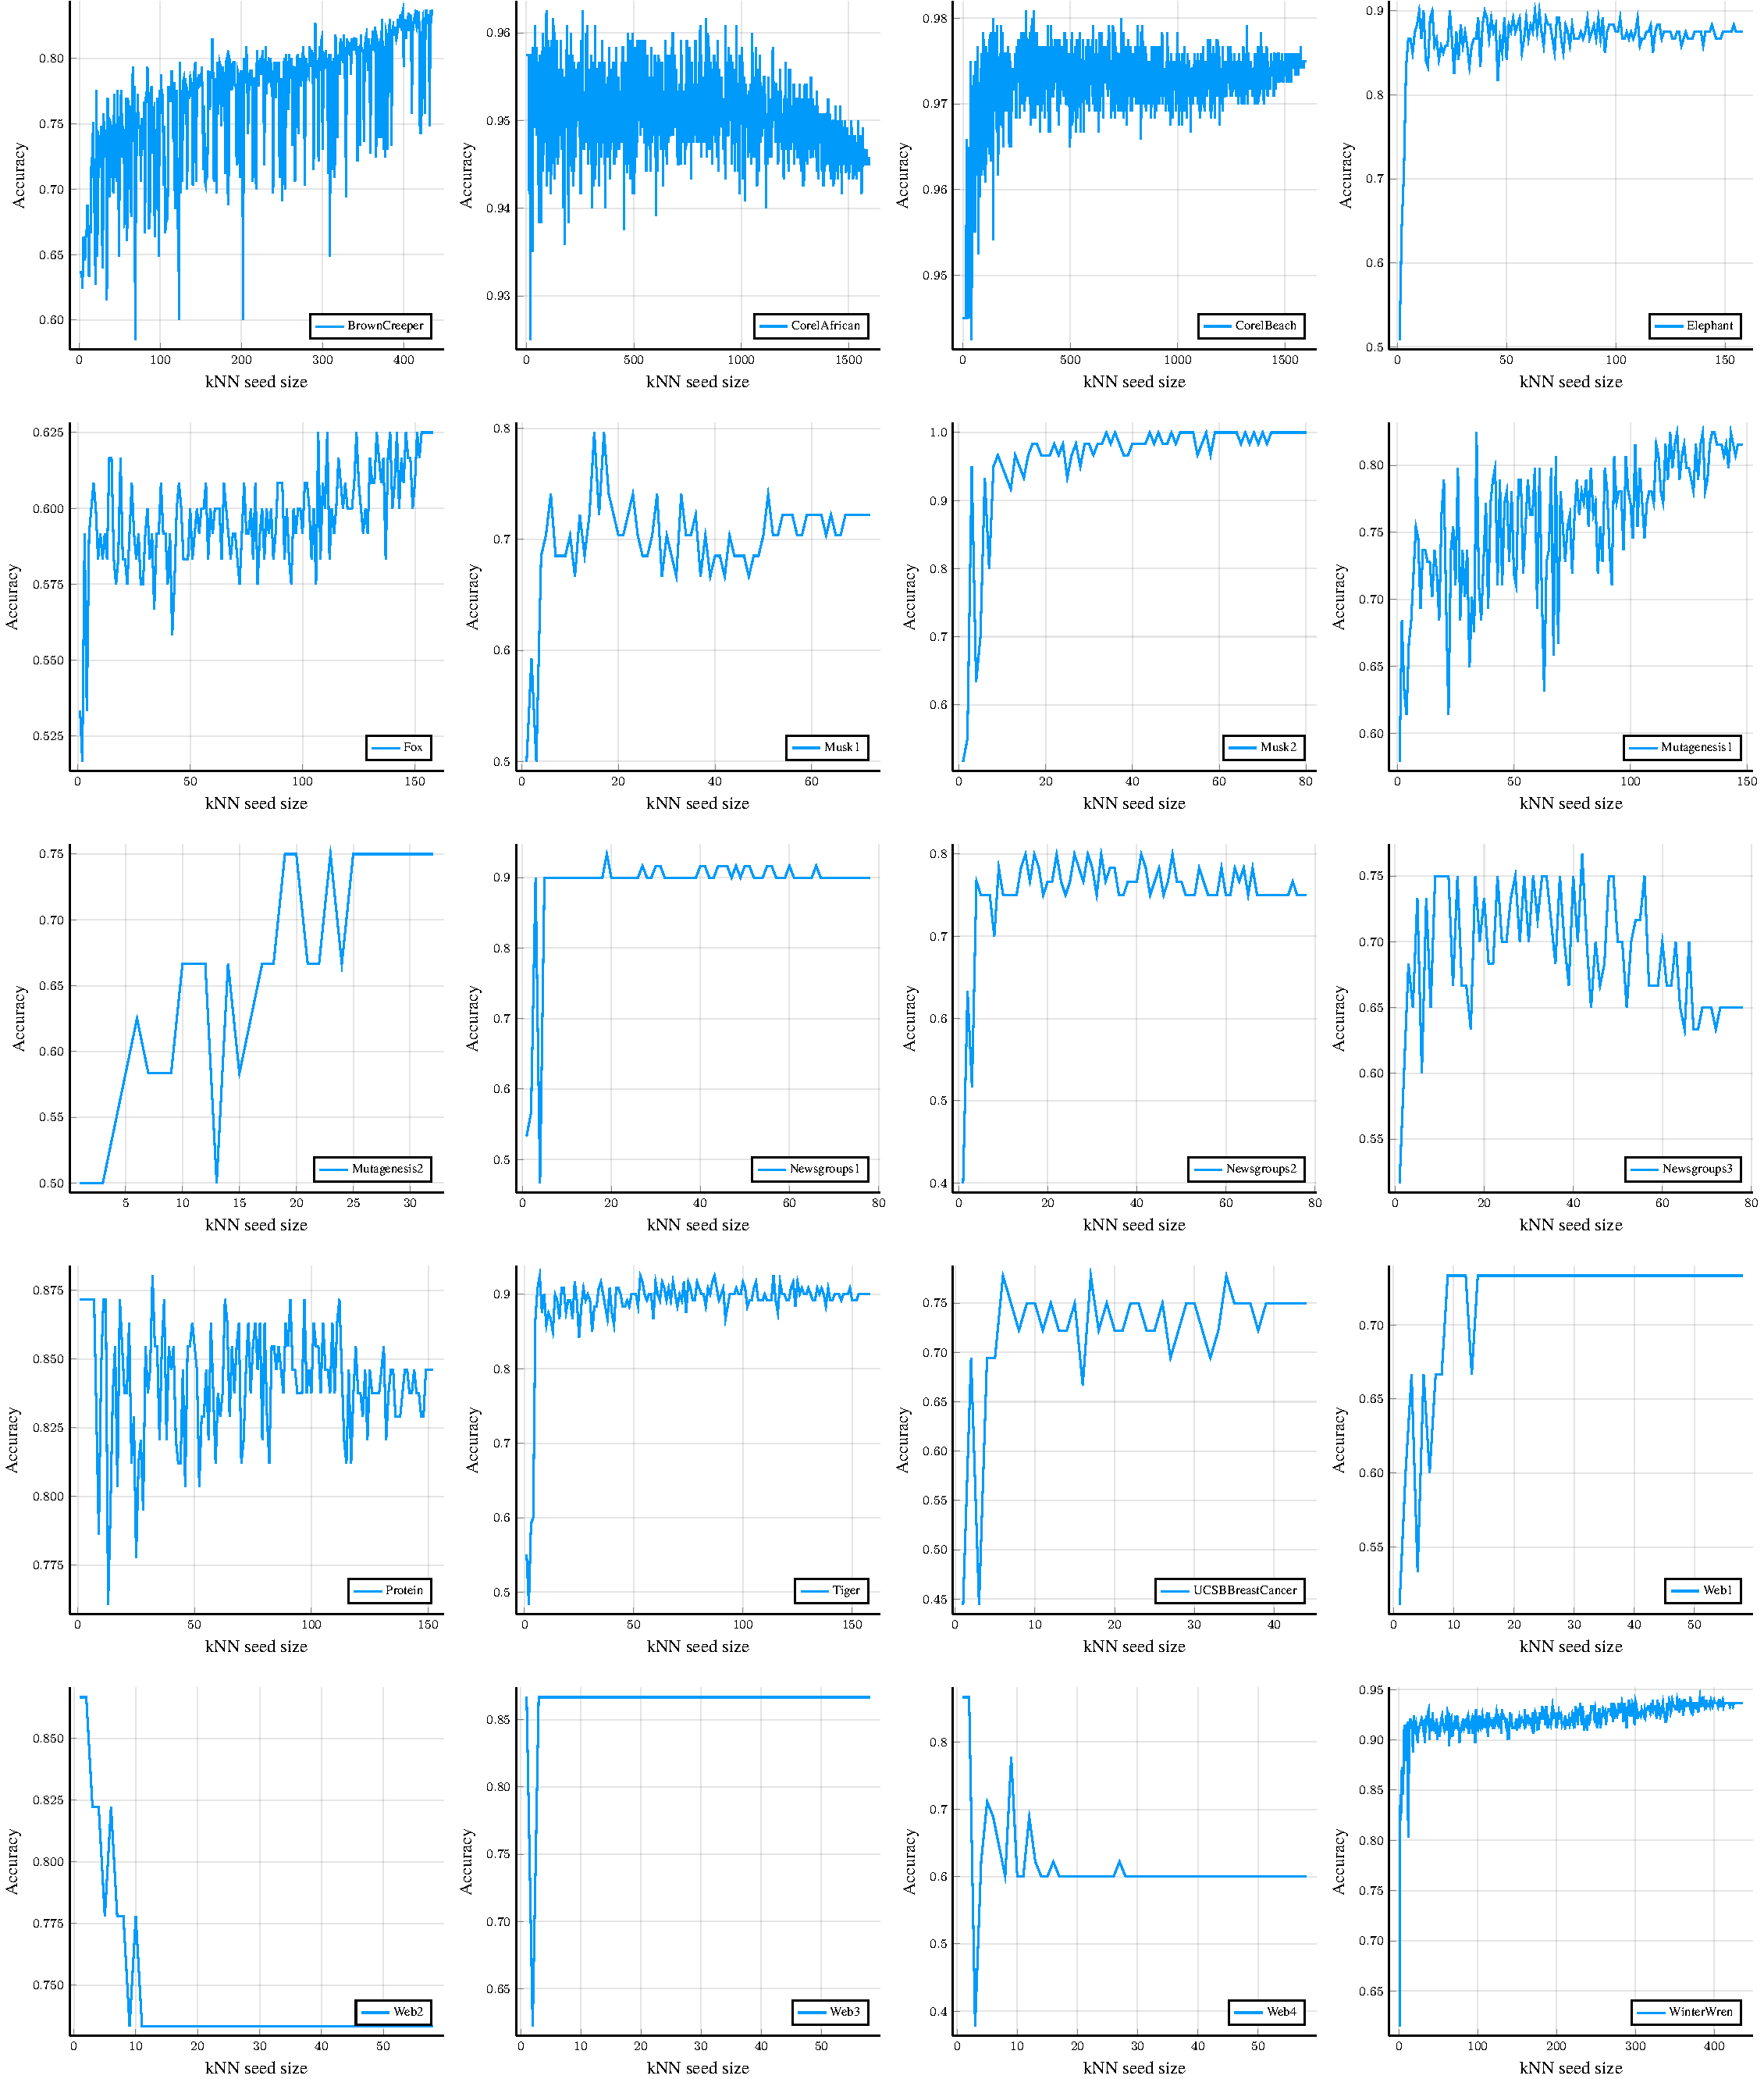
\includegraphics[width=\textwidth]{images/triplet-toy/kNN/triplet-toy-kNN.pdf}
  \caption{The accuracy of a kNN classifier built on the final embedding for triplet loss as a function of the number of samples used to seed it. Average of three runs.}\label{fig:triplet-toy-kNN}
\end{figure}

Figure \ref{fig:magnet-toy-ratio} shows the value of \( \mathrm{ratio} \left( \cdot \right) \) for magnet loss over the learning period. Figures \ref{fig:magnet-toy-accuracy} and \ref{fig:magnet-toy-kNN} show the accuracy of a kNN model built on the embedding.

\begin{figure}[h]
  \centering
  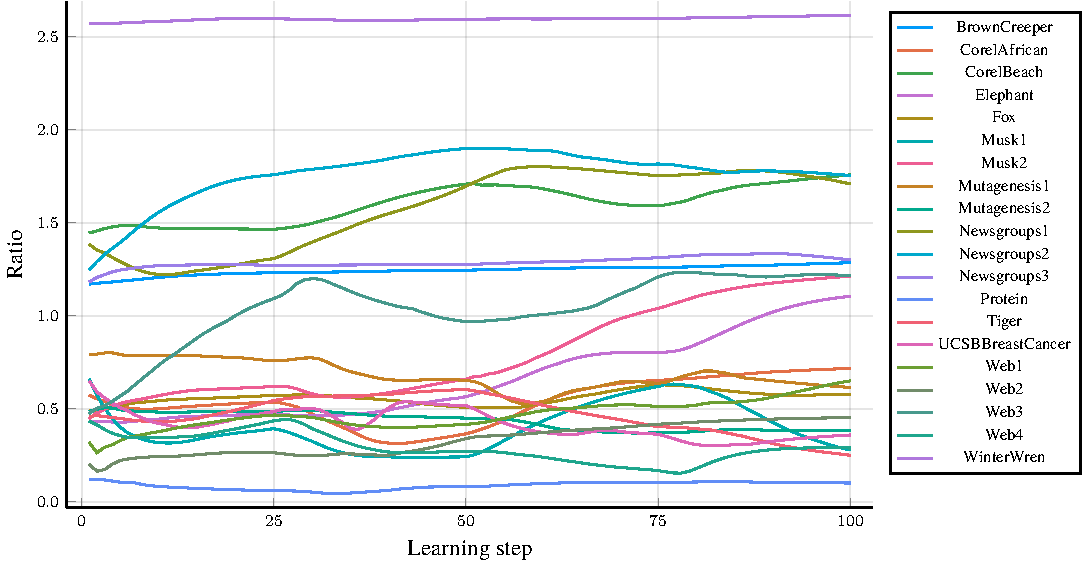
\includegraphics[width=\textwidth]{images/magnet-toy/ratio/magnet-toy-ratio.pdf}
  \caption{The value of \( \mathrm{ratio} \left( \cdot \right) \) for magnet loss over the learning period. Note the logarithmic scale on the \( y \) axis.}\label{fig:magnet-toy-ratio}
\end{figure}

\begin{figure}[h]
  \centering
  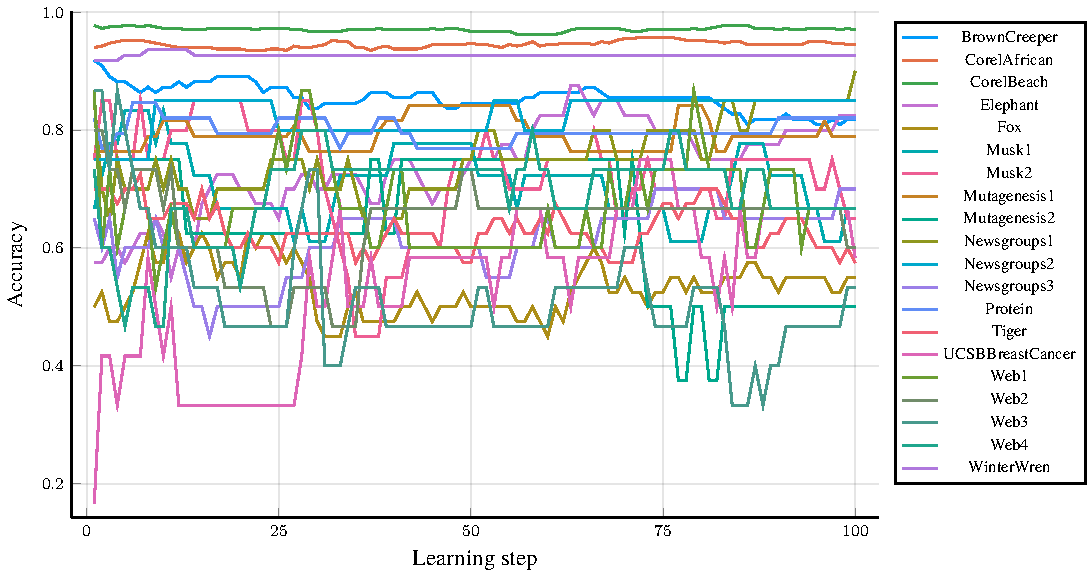
\includegraphics[width=\textwidth]{images/magnet-toy/accuracy/magnet-toy-accuracy.pdf}
  \caption{The accuracy of a kNN classifier built on the embedding for magnet loss over the learning period.}\label{fig:magnet-toy-accuracy}
\end{figure}

\begin{figure}[h]
  \centering
  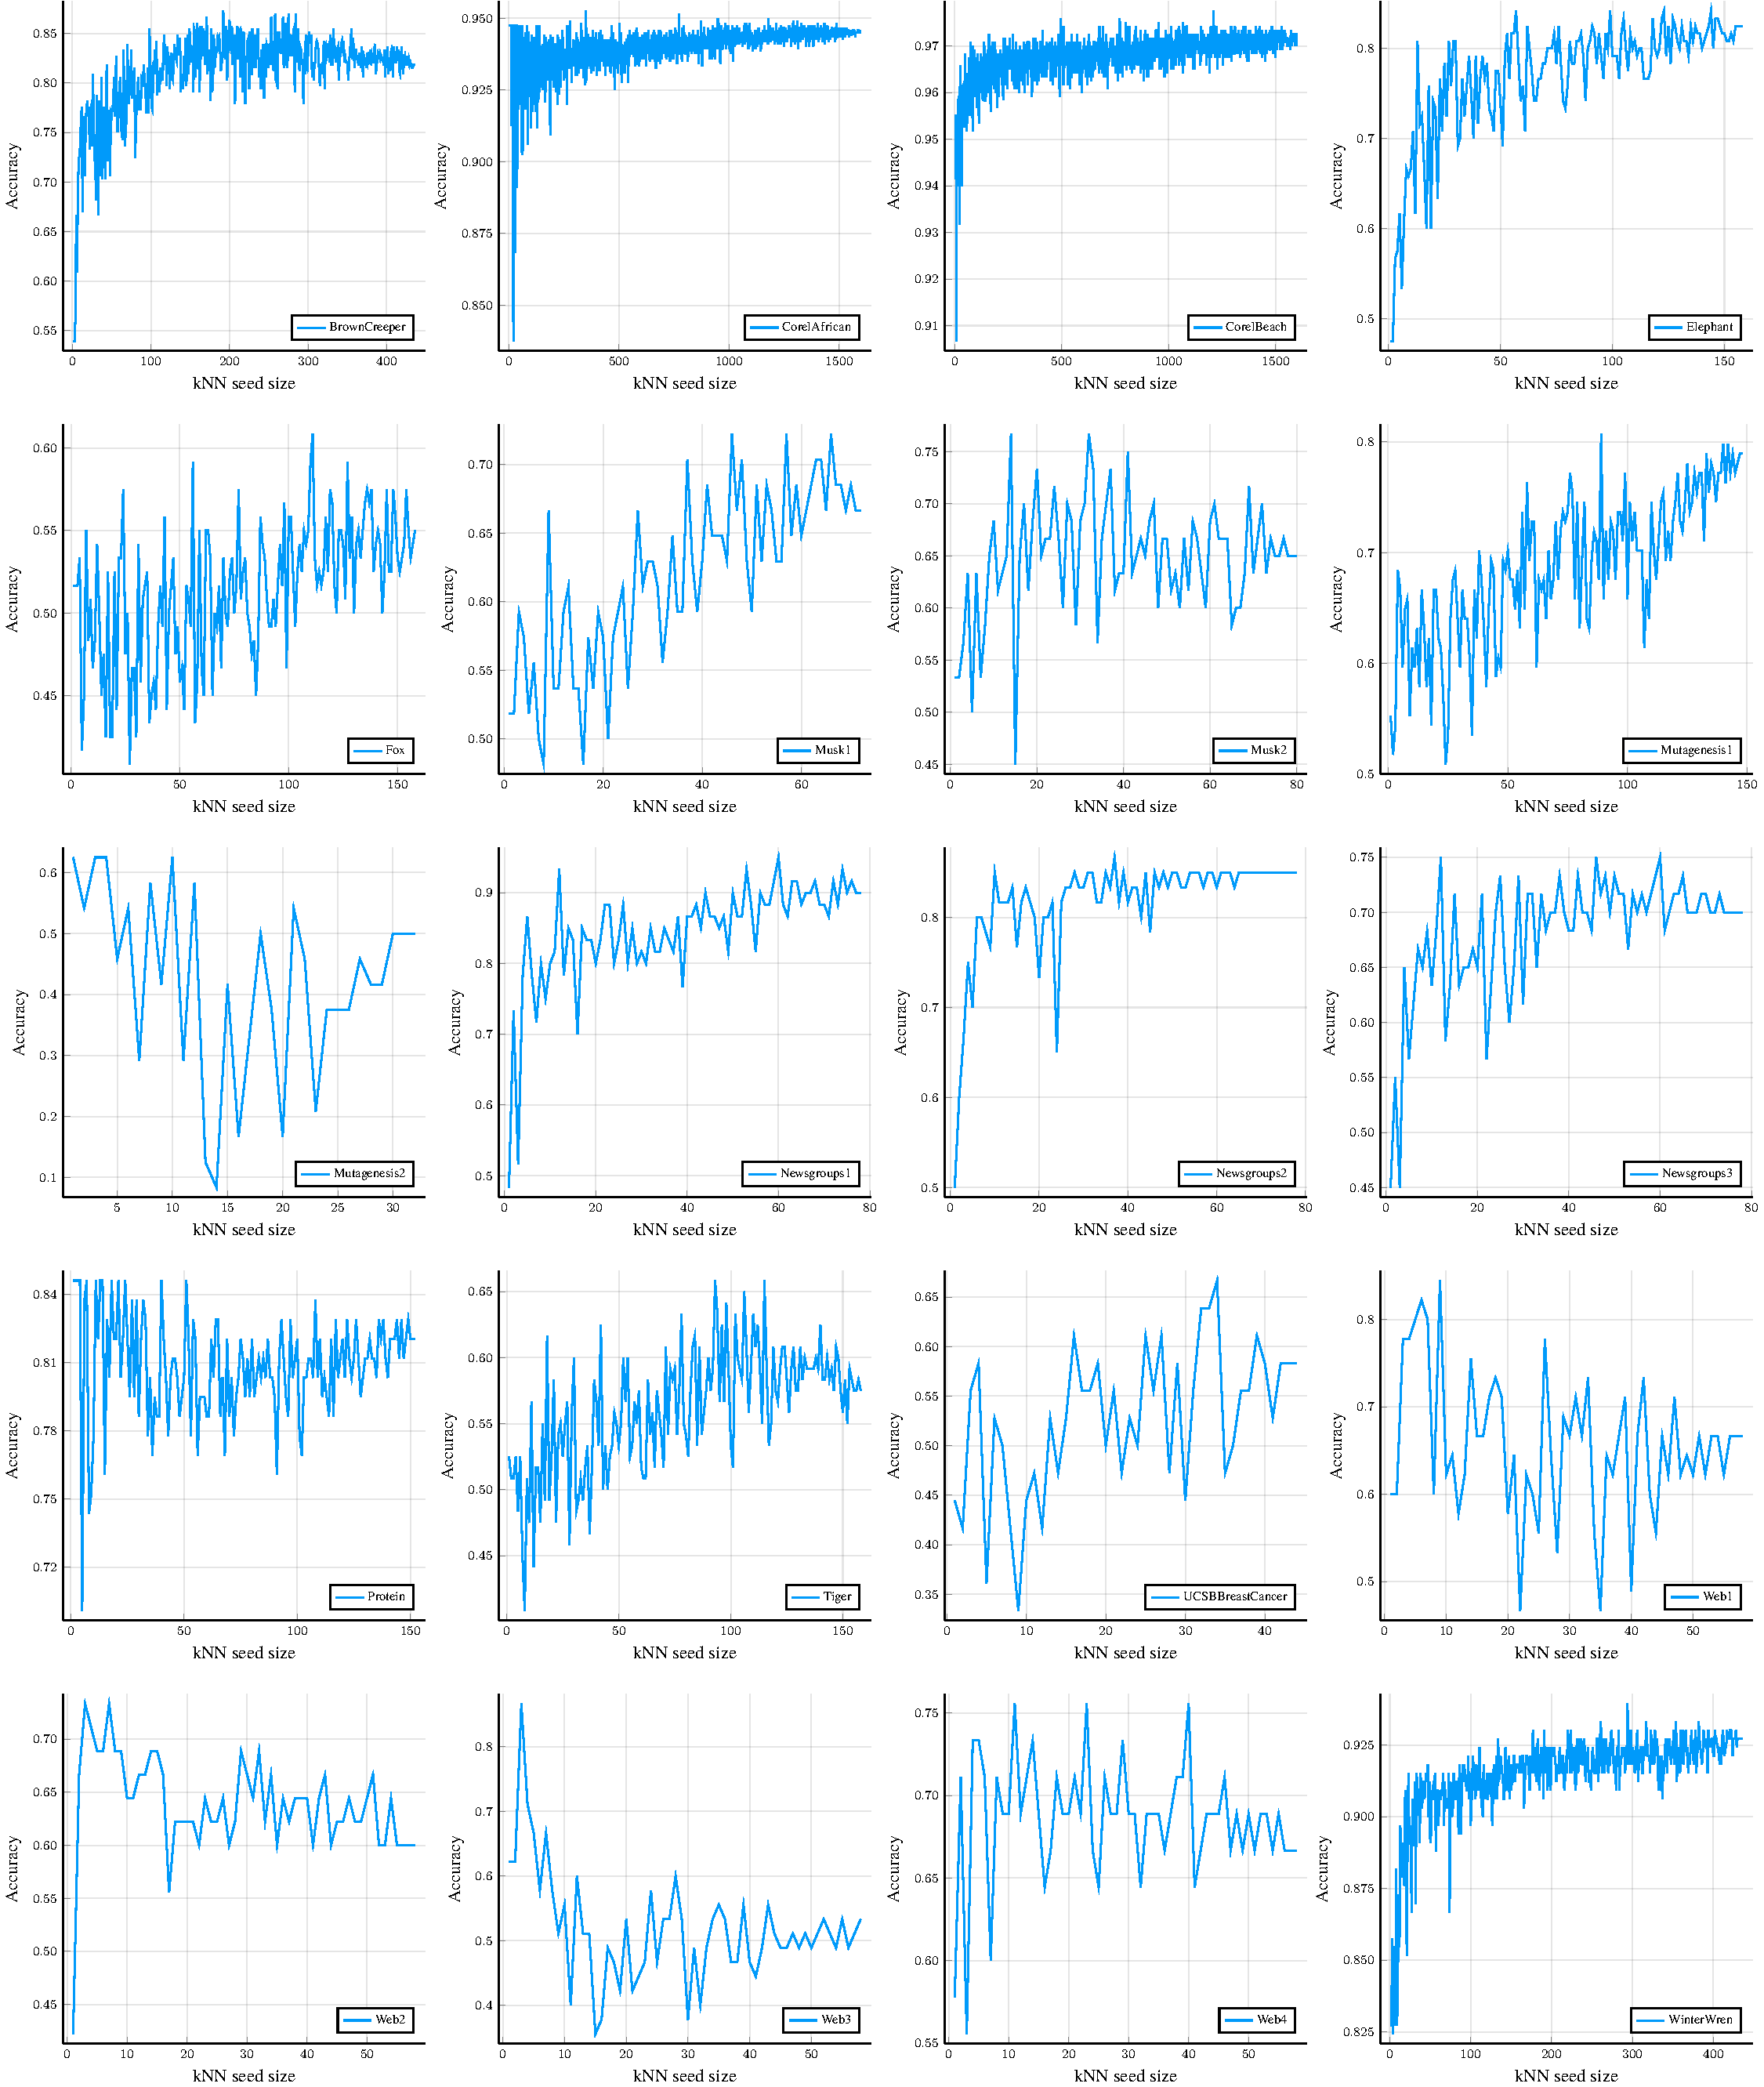
\includegraphics[width=\textwidth]{images/magnet-toy/kNN/magnet-toy-kNN.pdf}
  \caption{The accuracy of a kNN classifier built on the final embedding for magnet loss as a function of the number of samples used to seed it. Average of three runs.}\label{fig:magnet-toy-kNN}
\end{figure}

As can be seen from the figures, triplet loss is the clear winner among these 3 approaches as it is the only one which improves the metrics over the learning period. The other two methods show no clear improvement. With that said, however, the performance varies wildly between datasets. On the "Web" datasets, the value of \( \mathrm{ratio} \left( \cdot \right) \) quickly increases, but the accuracy of the kNN classifier remains fairly constant. This suggests that the embedding is quickly separating the different classes, but it does so in such a way that the kNN algorithm is not able to utilize this separation. This suggests that kNN might not be the right classification algorithm for this application.

Looking at the dependency of the accuracy on the size of the kNN seed data, some datasets clearly stand out as particularly hard for all of the methods (e.g. "Mutagenesis2"), while other have good results for all methods (e.g. "BrownCreeper"). Again, triplet loss is the clear winner as on most datasets it reaches its peak performance only with small amount of seed data.

Some of these findings go directly against the analysis presented in section \ref{sec:clustering-loss-comparison}, namely the prediction that magnet loss would be as good, if not better than triplet loss. The reason why it is not so may lie in the relative instability of the method, causing it to rapidly increase and the decrease all of the performance metrics.

\section{Magnet loss with self-tuning spectral clustering}\label{sec:magnet-spectral}

Figure \ref{fig:magnet-spectral} presents the difference between using K-means and self-tuning spectral clustering as the inner clustering algorithm in magnet loss.

\begin{figure}[h]
  \centering
  \begin{subfigure}[b]{0.49\textwidth}
    \centering
    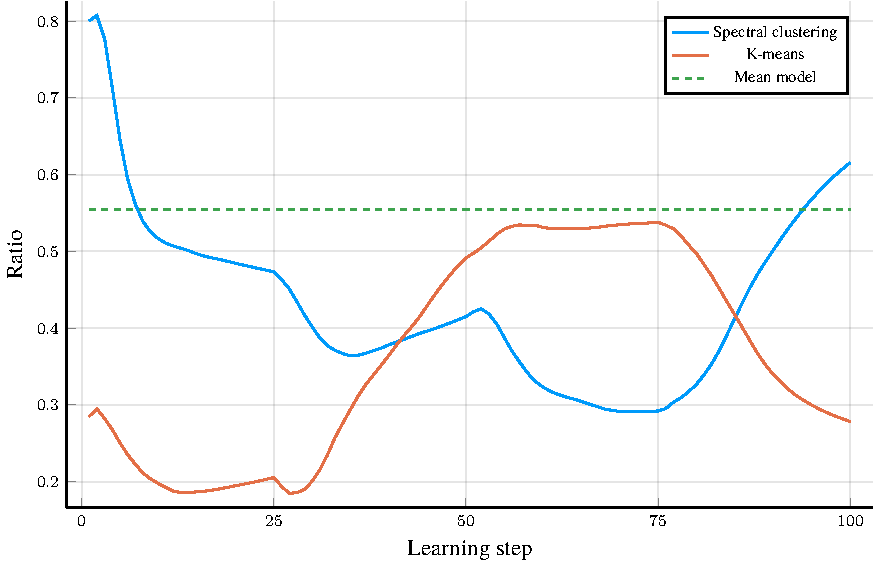
\includegraphics[width=\textwidth]{images/magnet-spectral/ratio/magnet-spectral-ratio.pdf}
    \caption{The value of \( \mathrm{ratio} \left( \cdot \right) \) over the learning period.}
  \end{subfigure}
  \hfill
  \begin{subfigure}[b]{0.49\textwidth}
    \centering
    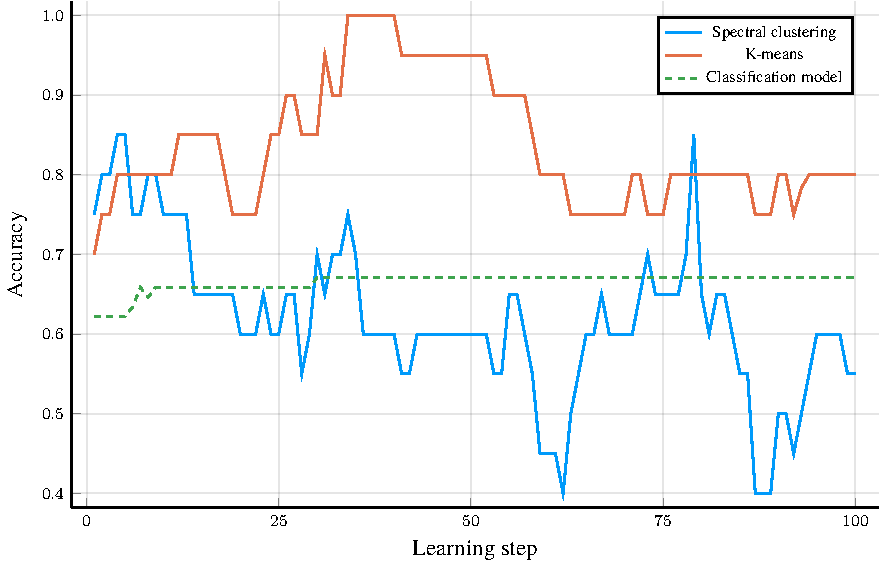
\includegraphics[width=\textwidth]{images/magnet-spectral/accuracy/magnet-spectral-accuracy.pdf}
    \caption{The accuracy of a kNN classifier built on the embedding over the learning period.}
  \end{subfigure}
  \caption{Comparison of the inner clustering algorithms for magnet loss.}\label{fig:magnet-spectral}
\end{figure}

As can be seen from the figures, the use of self-tuning spectral clustering brings no clear benefit to the performance of this method. The accuracy is lower then when the K-means algorithm was used, this can, however, be attributed to the instability of the method as a whole and may differ between runs.
